\documentclass{beamer}
\usetheme{tokitex}

\usepackage{tikz}
\usepackage{graphics}
\usepackage{multirow}
\usepackage{tabto}
\usepackage{xspace}
\usepackage{amsmath}
\usepackage{hyperref}
\usepackage{wrapfig}
\usepackage{mathtools}

\usepackage{tikz}
\usepackage{clrscode3e}
\usepackage{gensymb}

\usepackage[english,bahasa]{babel}
\newtranslation[to=bahasa]{Section}{Bagian}
\newtranslation[to=bahasa]{Subsection}{Subbagian}

\usepackage{listings, lstautogobble}
\usepackage{color}

\definecolor{dkgreen}{rgb}{0,0.6,0}
\definecolor{gray}{rgb}{0.5,0.5,0.5}
\definecolor{mauve}{rgb}{0.58,0,0.82}

\lstset{frame=tb,
  language=c++,
  aboveskip=0mm,
  belowskip=0mm,
  showstringspaces=false,
  columns=fullflexible,
  keepspaces=true,
  basicstyle={\small\ttfamily},
  numbers=none,
  numberstyle=\tiny\color{gray},
  keywordstyle=\color{blue},
  commentstyle=\color{dkgreen},
  stringstyle=\color{mauve},
  breaklines=true,
  breakatwhitespace=true,
  lineskip={-3pt}
}

\usepackage{caption}
\captionsetup[figure]{labelformat=empty}

\newcommand{\progTerm}[1]{\textbf{#1}}
\newcommand{\foreignTerm}[1]{\textit{#1}}
\newcommand{\newTerm}[1]{\alert{\textbf{#1}}}
\newcommand{\emp}[1]{\alert{#1}}
\newcommand{\statement}[1]{"#1"}

\newcommand{\floor}[1]{\lfloor #1 \rfloor}
\newcommand{\ceil}[1]{\lceil #1 \rceil}
\newcommand{\abs}[1]{\left\lvert#1\right\rvert}
\newcommand{\norm}[1]{\left\lVert#1\right\rVert}

% Getting tired of writing \foreignTerm all the time
\newcommand{\farray}{\foreignTerm{array}\xspace}
\newcommand{\fArray}{\foreignTerm{Array}\xspace}
\newcommand{\foverhead}{\foreignTerm{overhead}\xspace}
\newcommand{\fOverhead}{\foreignTerm{Overhead}\xspace}
\newcommand{\fsubarray}{\foreignTerm{subarray}\xspace}
\newcommand{\fSubarray}{\foreignTerm{Subarray}\xspace}
\newcommand{\fbasecase}{\foreignTerm{base case}\xspace}
\newcommand{\fBasecase}{\foreignTerm{Base case}\xspace}
\newcommand{\ftopdown}{\foreignTerm{top-down}\xspace}
\newcommand{\fTopdown}{\foreignTerm{Top-down}\xspace}
\newcommand{\fbottomup}{\foreignTerm{bottom-up}\xspace}
\newcommand{\fBottomup}{\foreignTerm{Bottom-up}\xspace}
\newcommand{\fpruning}{\foreignTerm{pruning}\xspace}
\newcommand{\fPruning}{\foreignTerm{Pruning}\xspace}

\newcommand{\fgraph}{\foreignTerm{graph}\xspace}
\newcommand{\fGraph}{\foreignTerm{Graph}\xspace}
\newcommand{\froot}{\foreignTerm{root}\xspace}
\newcommand{\fRoot}{\foreignTerm{Root}\xspace}
\newcommand{\fnode}{\foreignTerm{node}\xspace}
\newcommand{\fNode}{\foreignTerm{Node}\xspace}
\newcommand{\fedge}{\foreignTerm{edge}\xspace}
\newcommand{\fEdge}{\foreignTerm{Edge}\xspace}
\newcommand{\fcycle}{\foreignTerm{cycle}\xspace}
\newcommand{\fCycle}{\foreignTerm{Cycle}\xspace}
\newcommand{\fdegree}{\foreignTerm{degree}\xspace}
\newcommand{\fDegree}{\foreignTerm{Degree}\xspace}
\newcommand{\fadjacencylist}{\foreignTerm{adjacency list}\xspace}
\newcommand{\fAdjacencylist}{\foreignTerm{Adjacency list}\xspace}
\newcommand{\fadjacencymatrix}{\foreignTerm{adjacency matrix}\xspace}
\newcommand{\fAdjacencymatrix}{\foreignTerm{Adjacency matrix}\xspace}
\newcommand{\fedgelist}{\foreignTerm{edge list}\xspace}
\newcommand{\fEdgelist}{\foreignTerm{Edge list}\xspace}
\newcommand{\flist}{\foreignTerm{list}\xspace}
\newcommand{\fList}{\foreignTerm{List}\xspace}
\newcommand{\fgraphtraversal}{\foreignTerm{graph traversal}\xspace}
\newcommand{\fGraphtraversal}{\foreignTerm{Graph traversal}\xspace}
\newcommand{\ftree}{\foreignTerm{tree}\xspace}
\newcommand{\fTree}{\foreignTerm{Tree}\xspace}
\newcommand{\fsubtree}{\foreignTerm{subtree}\xspace}
\newcommand{\fSubtree}{\foreignTerm{Subtree}\xspace}
\newcommand{\fparent}{\foreignTerm{parent}\xspace}
\newcommand{\fParent}{\foreignTerm{Parent}\xspace}
\newcommand{\fsibling}{\foreignTerm{sibling}\xspace}
\newcommand{\fSibling}{\foreignTerm{Sibling}\xspace}
\newcommand{\fpath}{\foreignTerm{path}\xspace}
\newcommand{\fPath}{\foreignTerm{Path}\xspace}
\newcommand{\fconnectedcomponent}{\foreignTerm{connected component}\xspace}
\newcommand{\fConnectedcomponent}{\foreignTerm{Connected component}\xspace}
\newcommand{\fbridge}{\foreignTerm{bridge}\xspace}
\newcommand{\fBridge}{\foreignTerm{Bridge}\xspace}
\newcommand{\farticulationpoint}{\foreignTerm{articulation point}\xspace}
\newcommand{\fArticulationpoint}{\foreignTerm{Articulation point}\xspace}
\newcommand{\ftreeedge}{\foreignTerm{tree edge}\xspace}
\newcommand{\fTreeedge}{\foreignTerm{Tree edge}\xspace}
\newcommand{\fbackedge}{\foreignTerm{back edge}\xspace}
\newcommand{\fBackedge}{\foreignTerm{Back edge}\xspace}
\newcommand{\fforwardedge}{\foreignTerm{forward edge}\xspace}
\newcommand{\fForwardedge}{\foreignTerm{Forward edge}\xspace}
\newcommand{\fcrossedge}{\foreignTerm{cross edge}\xspace}
\newcommand{\fCrossedge}{\foreignTerm{Cross edge}\xspace}
\newcommand{\fdiscoverytime}{\foreignTerm{discovery time}\xspace}
\newcommand{\fDiscoverytime}{\foreignTerm{Discovery time}\xspace}
\newcommand{\flowlink}{\foreignTerm{low link}\xspace}
\newcommand{\fLowlink}{\foreignTerm{Low link}\xspace}
\newcommand{\fstack}{\foreignTerm{stack}\xspace}
\newcommand{\fStack}{\foreignTerm{Stack}\xspace}
\newcommand{\for}{\foreignTerm{or}\xspace}
\newcommand{\fOr}{\foreignTerm{Or}\xspace}
\newcommand{\fand}{\foreignTerm{and}\xspace}
\newcommand{\fAnd}{\foreignTerm{And}\xspace}
\newcommand{\fcentroid}{\foreignTerm{centroid}\xspace}
\newcommand{\fCentroid}{\foreignTerm{Centroid}\xspace}

\newcommand{\fDivideAndConquer}{\foreignTerm{Divide and conquer}\xspace}
\newcommand{\fdivideAndConquer}{\foreignTerm{divide and conquer}\xspace}
\newcommand{\fMergeSort}{\foreignTerm{Merge sort}\xspace}
\newcommand{\fmergeSort}{\foreignTerm{merge sort}\xspace}
\newcommand{\fQuickSort}{\foreignTerm{Quicksort}\xspace}
\newcommand{\fquickSort}{\foreignTerm{quicksort}\xspace}
\newcommand{\fpivot}{\foreignTerm{pivot}\xspace}
\newcommand{\fPivot}{\foreignTerm{Pivot}\xspace}
\newcommand{\fbruteForce}{\foreignTerm{brute force}\xspace}
\newcommand{\fBruteForce}{\foreignTerm{Brute force}\xspace}
\newcommand{\fCompleteSearch}{\foreignTerm{complete search}\xspace}
\newcommand{\fExhaustiveSearch}{\foreignTerm{exhaustive search}\xspace}
\newcommand{\fbinarySearch}{\foreignTerm{binary search}\xspace}
\newcommand{\fBinarySearch}{\foreignTerm{Binary search}\xspace}
\newcommand{\fternarySearch}{\foreignTerm{ternary search}\xspace}
\newcommand{\fTernarySearch}{\foreignTerm{Ternary search}\xspace}
\newcommand{\funimodal}{\foreignTerm{unimodal}\xspace}
\newcommand{\fUnimodal}{\foreignTerm{Unimodal}\xspace}
\newcommand{\fGreedy}{\foreignTerm{Greedy}\xspace}
\newcommand{\fgreedy}{\foreignTerm{greedy}\xspace}
\newcommand{\fgreedyChoice}{\foreignTerm{greedy choice}\xspace}
\newcommand{\fGreedyChoice}{\foreignTerm{Greedy choice}\xspace}

\newcommand{\fdp}{\foreignTerm{dynamic programming}\xspace}
\newcommand{\fDp}{\foreignTerm{Dynamic programming}\xspace}
\newcommand{\fbitmask}{\foreignTerm{bitmask}\xspace}
\newcommand{\fBitmask}{\foreignTerm{Bitmask}\xspace}
\newcommand{\fstate}{\foreignTerm{state}\xspace}
\newcommand{\fState}{\foreignTerm{State}\xspace}
\newcommand{\fsubmask}{\foreignTerm{submask}\xspace}
\newcommand{\fSubmask}{\foreignTerm{Submask}\xspace}

\newcommand{\pheap}{\foreignTerm{heap}\xspace}
\newcommand{\pHeap}{\foreignTerm{Heap}\xspace}
\newcommand{\pBinaryHeap}{\foreignTerm{Binary Heap}\xspace}
\newcommand{\pbinaryHeap}{\foreignTerm{binary heap}\xspace}
\newcommand{\pHeapsort}{\foreignTerm{Heapsort}\xspace}
\newcommand{\pheapsort}{\foreignTerm{heapsort}\xspace}
\newcommand{\pdjs}{\foreignTerm{disjoint set}\xspace}
\newcommand{\pDjs}{\foreignTerm{Disjoint set}\xspace}

\newcommand{\fdotProduct}{\foreignTerm{dot product}\xspace}
\newcommand{\fDotProduct}{\foreignTerm{Dot product}\xspace}
\newcommand{\fcrossProduct}{\foreignTerm{cross product}\xspace}
\newcommand{\fCrossProduct}{\foreignTerm{Cross product}\xspace}
\newcommand{\fconvexHull}{\foreignTerm{convex hull}\xspace}
\newcommand{\fConvexHull}{\foreignTerm{Convex hull}\xspace}
\newcommand{\fgrahamScan}{\foreignTerm{graham scan}\xspace}
\newcommand{\fGrahamScan}{\foreignTerm{Graham scan}\xspace}
\newcommand{\flineSweep}{\foreignTerm{line sweep}\xspace}
\newcommand{\fLineSweep}{\foreignTerm{Line sweep}\xspace}

\newcommand{\fset}{\foreignTerm{set}\xspace}
\newcommand{\fSet}{\foreignTerm{Set}\xspace}
\newcommand{\fprefixSum}{\foreignTerm{prefix sum}\xspace}
\newcommand{\fPrefixSum}{\foreignTerm{Prefix sum}\xspace}
\newcommand{\ffenwickTree}{\foreignTerm{fenwick tree}\xspace}
\newcommand{\fFenwickTree}{\foreignTerm{Fenwick tree}\xspace}
\newcommand{\frangeSumQuery}{\foreignTerm{range sum query}\xspace}
\newcommand{\fRangeSumQuery}{\foreignTerm{Range sum query}\xspace}
\newcommand{\fquery}{\foreignTerm{query}\xspace}
\newcommand{\fQuery}{\foreignTerm{Query}\xspace}
\newcommand{\fsegmentTree}{\foreignTerm{segment tree}\xspace}
\newcommand{\fSegmentTree}{\foreignTerm{Segment tree}\xspace}
\newcommand{\fbinaryTree}{\foreignTerm{binary tree}\xspace}
\newcommand{\fBinaryTree}{\foreignTerm{Binary tree}\xspace}
\newcommand{\flazyPropagation}{\foreignTerm{lazy propagation}\xspace}
\newcommand{\fLazyPropagation}{\foreignTerm{Lazy propagation}\xspace}
\newcommand{\fsparseTable}{\foreignTerm{sparse table}\xspace}
\newcommand{\fSparseTable}{\foreignTerm{Sparse table}\xspace}

\newcommand{\ftrail}{\foreignTerm{trail}\xspace}
\newcommand{\fTrail}{\foreignTerm{Trail}\xspace}
\newcommand{\feulerTour}{\foreignTerm{euler tour}\xspace}
\newcommand{\fEulerTour}{\foreignTerm{Euler tour}\xspace}
\newcommand{\feulerTourTree}{\foreignTerm{euler tour tree}\xspace}
\newcommand{\fEulerTourTree}{\foreignTerm{Euler tour tree}\xspace}

\newcommand{\fmaxflow}{\foreignTerm{maximum flow}\xspace}
\newcommand{\fMaxflow}{\foreignTerm{Maximum flow}\xspace}
\newcommand{\fmincut}{\foreignTerm{minimum cut}\xspace}
\newcommand{\fMincut}{\foreignTerm{Minimum cut}\xspace}
\newcommand{\fflow}{\foreignTerm{flow}\xspace}
\newcommand{\fFlow}{\foreignTerm{Flow}\xspace}
\newcommand{\fsource}{\foreignTerm{source}\xspace}
\newcommand{\fSource}{\foreignTerm{Source}\xspace}
\newcommand{\fsink}{\foreignTerm{sink}\xspace}
\newcommand{\fSink}{\foreignTerm{Sink}\xspace}
\newcommand{\fbackEdge}{\foreignTerm{back-edge}\xspace}
\newcommand{\fBackEdge}{\foreignTerm{Back-edge}\xspace}
\newcommand{\fresidualCapacity}{\foreignTerm{residual capacity}\xspace}
\newcommand{\fResidualCapacity}{\foreignTerm{Residual capacity}\xspace}
\newcommand{\fbottleneck}{\foreignTerm{bottleneck}\xspace}
\newcommand{\fBottleneck}{\foreignTerm{Bottleneck}\xspace}
\newcommand{\faugmentingPath}{\foreignTerm{augmenting path}\xspace}
\newcommand{\fAugmentingPath}{\foreignTerm{Augmenting path}\xspace}


\title{Perkenalan Graf}
\author{Tim Olimpiade Komputer Indonesia}
\date{}

\usepackage{verbatim}
\usepackage{multicol}
\lstset{escapeinside={<@}{@>},belowskip=\baselineskip}
\definecolor{mygreen}{rgb}{0, 0.597, 0.199}

\begin{document}

\begin{frame}
\titlepage
\end{frame}

\begin{frame}
\frametitle{Pendahuluan}
Melalui dokumen ini, kalian akan:
\begin{itemize}
  \item Mengenal konsep dan terminologi graf.
  \item Mengetahui jenis-jenis graf.
  \item Mengenal representasi graf pada pemrograman.
  \item Mengenal metode-metode yang digunakan dalam graf.
\end{itemize}
\end{frame}

\begin{frame}
\frametitle{Motivasi}
\begin{itemize}
  \item Diberikan sebuah struktur kota dan jalan.
  \item Terdapat $V$ kota, dan $E$ ruas jalan.
  \item Setiap ruas jalan menghubungkan dua kota.
  \item Diberikan kota awal, tentukan berapa banyak ruas jalan paling sedikit yang perlu dilalui untuk mencapai suatu kota tujuan!
\end{itemize}
\end{frame}

\begin{frame}
\frametitle{Pertanyaan}
\begin{center}
  \large Bagaimana cara merepresentasikan struktur perkotaan dan jalan pada pemrograman?
\end{center}
\end{frame}

\section{Perkenalan Graf}
\frame{\sectionpage}

\begin{frame}
\frametitle{Mengenal Graf}
Graf adalah struktur yang terdiri dari \newTerm{\fnode/\foreignTerm{vertex}} dan \newTerm{\fedge.}\newline

\fNode direpresentasikan dengan bentuk lingkaran dan \fedge direpresentasikan dengan bentuk garis pada ilustrasi berikut:

\begin{figure}
  \centering
  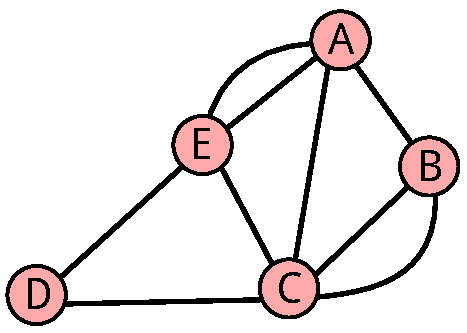
\includegraphics[width=4 cm]{asset/graph.pdf}
\end{figure}
\end{frame}

\begin{frame}
\frametitle{Mengenal Graf (lanj.)}
\begin{itemize}
  \item \fEdge merupakan penghubung antar \fnode.
  \item \alert{\fDegree} suatu \fnode merupakan jumlah \fedge yang terhubung pada \fnode tersebut
  \item Pada contoh ilustrasi berikut, \fdegree \fnode A = 4, \fdegree \fnode B = 3, dan \fdegree \fnode C = 5.
\end{itemize}
\begin{figure}
  \centering
  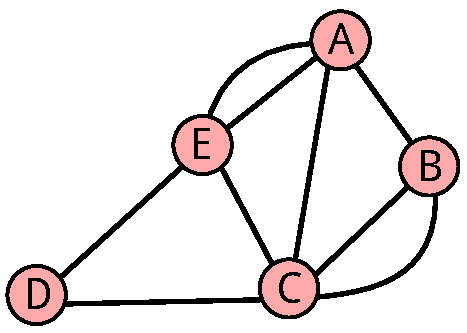
\includegraphics[width=4 cm]{asset/graph.pdf}
\end{figure}
\end{frame}

\begin{frame}
\frametitle{Jenis Graf}
Berdasarkan hubungan antar \fnode:
\begin{itemize}
  \item \newTerm{Graf tak berarah}: \fedge dari A ke B dapat ditelusuri dari A ke B dan B ke A. 
  \item \newTerm{Graf berarah}: \fedge dari A ke B hanya dapat ditelusuri dari dari A ke B.
\end{itemize}
\begin{figure}
  \centering
  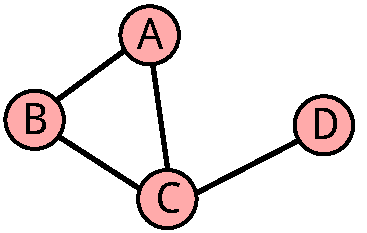
\includegraphics[width=4 cm]{asset/unweighted-undirected.pdf}
  \ \ \ \ \ \ % If this works, this ain't stupid
  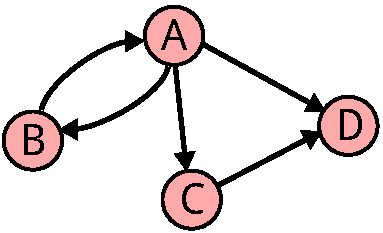
\includegraphics[width=4 cm]{asset/unweighted-directed.pdf}
  
  Graf tak berarah dan graf berarah
\end{figure}
\end{frame}

\begin{frame}
\frametitle{Jenis Graf (lanj.)}
Berdasarkan bobot dari \fedge:
\begin{itemize}
  \item \newTerm{Graf tak berbobot}, yaitu graf dengan \fedge yang bobotnya seragam dan hanya bermakna terdapat hubungan antar \fnode.
  \item \newTerm{Graf berbobot}, yaitu graf dengan \fedge yang dapat memiliki bobot berbeda-beda. Bobot pada \fedge ini bisa jadi berupa biaya, jarak, atau waktu yang harus ditempuh jika menggunakan \fedge tersebut.
\end{itemize}
\begin{figure}
  \centering
  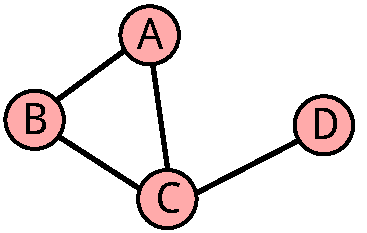
\includegraphics[width=4 cm]{asset/unweighted-undirected.pdf}
  \ \ \ \ \ \ % If this works, this ain't stupid
  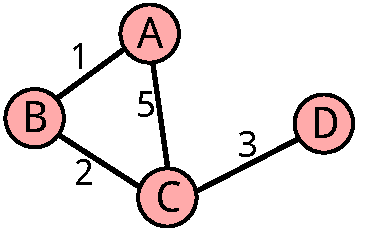
\includegraphics[width=4 cm]{asset/weighted-undirected.pdf}
  
  Graf tak berbobot dan graf berbobot
\end{figure}
\end{frame}

\begin{frame}
\frametitle{Jenis Graf (lanj.)}
Tentu saja, suatu graf dapat memiliki kombinasi dari sifat-sifat tersebut.

Misalnya graf berbobot berarah:
\newline
\begin{figure}
  \centering
  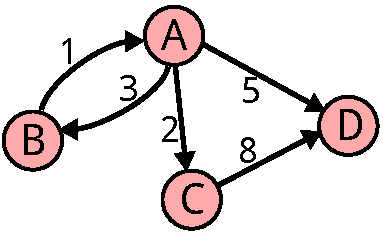
\includegraphics[width=5 cm]{asset/weighted-directed.pdf}
\end{figure}
\end{frame}

\begin{frame}
\frametitle{Representasi Graf pada Pemrograman}

\begin{itemize}
  \item Dalam pemrograman, dibutuhkan sebuah struktur agar data mengenai graf dapat disimpan dan diolah.
  \item Representasi yang akan kita pelajari adalah \fadjacencymatrix, \fadjacencylist, dan \fedgelist.
  \item Masing-masing representasi memiliki keuntungan dan kerugiannya.
  \item Penggunaan representasi graf bergantung dengan masalah yang sedang dihadapi.
\end{itemize}
\end{frame}

\begin{frame}
\frametitle{Adjacency Matrix}
\begin{itemize}
  \item Kita akan menggunakan matriks dengan ukuran $N \times N$ dengan $N$ merupakan banyaknya \fnode.
  \item Pada graf tidak berbobot:
  \begin{itemize}
    \item Jika terdapat \fedge dari A ke B, maka $matrix[A][B] = 1$. 
    \item Jika tidak ada, maka $matrix[A][B] = 0$.
  \end{itemize}
\end{itemize}

\begin{center}
\begin{multicols}{2}
  $\begin{array}{c|cccc}
      & A & B & C & D \\ \hline
    A & 0 & 1 & 1 & 1 \\
    B & 1 & 0 & 0 & 0 \\
    C & 0 & 0 & 0 & 1 \\
    D & 0 & 0 & 0 & 0
  \end{array}$
  \break
  \begin{figure}
    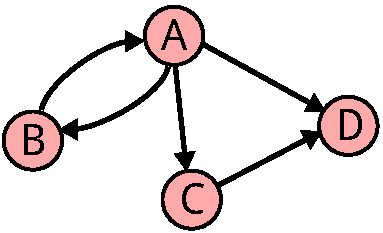
\includegraphics[width=4 cm]{asset/unweighted-directed.pdf}
  \end{figure}
\end{multicols} 
\end{center}
\end{frame}

\begin{frame}
\frametitle{Adjacency Matrix (lanj.)}
\begin{itemize}
  \item Pada graf berbobot:
  \begin{itemize}
    \item Jika terdapat \fedge dari A ke B dengan bobot w, maka $matrix[A][B] = w$. 
    \item Jika tidak ada, maka dapat ditulis $matrix[A][B] = \infty$.
  \end{itemize}
\end{itemize}

\begin{center}
\begin{multicols}{2}
  $\begin{array}{c|cccc}
      & A & B & C & D \\ \hline
    A & \infty & 3 & 2 & 5 \\
    B & 1 & \infty & \infty & \infty \\
    C & \infty & \infty & \infty & 8 \\
    D & \infty & \infty & \infty & \infty
  \end{array}$
  \break
  \begin{figure}
    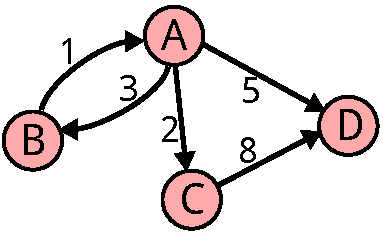
\includegraphics[width=4 cm]{asset/weighted-directed.pdf}
  \end{figure}
\end{multicols} 
\end{center}
\end{frame}

\begin{frame}
\frametitle{Analisis Adjacency Matrix}
\begin{itemize}
  \item Pada graf tak berarah, \fadjacencymatrix simetris terhadap diagonalnya.
  \item Representasi ini mudah diimplementasikan.
  \item Menambah atau menghapus \fedge dapat dilakukan dalam $O(1)$.
  \item Untuk memeriksa apakah dua \fnode terhubung juga dapat dilakukan dalam $O(1)$.
  \item Untuk mendapatkan daftar tetangga dari suatu \fnode, dapat dilakukan iterasi $O(V)$, dengan $V$ adalah banyaknya \fnode.
\end{itemize}
\end{frame}

\begin{frame}
\frametitle{Kekurangan Adjacency Matrix}
\begin{itemize}
  \item Kekurangan dari representasi ini adalah boros memori.
  \item Memori yang dibutuhkan selalu $O(V^2)$, tidak dapat digunakan untuk graf dengan \fnode mencapai ratusan ribu.
  \item Jika banyaknya \fedge jauh lebih sedikit dari $O(V^2)$, maka banyak memori yang terbuang.
\end{itemize}
\end{frame}

\begin{frame}
\frametitle{Adjacency List}
\begin{itemize}
  \item Merupakan salah satu alternatif representasi graf.
  \item Untuk setiap \fnode, buat sebuah \flist yang berisi keterangan mengenai tetangga \fnode tersebut.
  \item Misalnya untuk graf tak berbobot, kita cukup menyimpan \fnode-\fnode tetangga untuk setiap \fnode.
\end{itemize}
\begin{center}
\begin{multicols}{2}
  $\begin{array}{r|l}
    A & [B, C, D] \\
    B & [A] \\
    C & [D] \\
    D & [\ ]
  \end{array}$
  \break
  \begin{figure}
    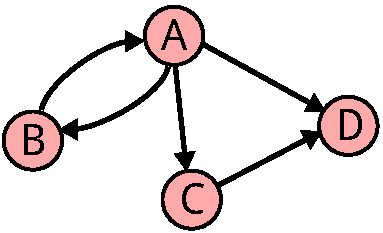
\includegraphics[width=4 cm]{asset/unweighted-directed.pdf}
  \end{figure}
\end{multicols} 
\end{center}
\end{frame}

\begin{frame}
\frametitle{Adjacency List (lanj.)}
\begin{itemize}
  \item Untuk graf berbobot, kita dapat menyimpan \fnode-\fnode tetangga beserta bobotnya.
\end{itemize}
\begin{center}
\begin{multicols}{2}
  $\begin{array}{r|l}
    A & [<B,3> , <C,2>, <D,5>] \\
    B & [<A,1>] \\
    C & [<D,8>] \\
    D & [\ ]
  \end{array}$
  \break
  \begin{figure}
    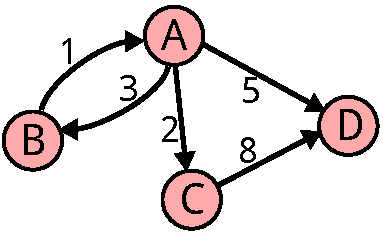
\includegraphics[width=4 cm]{asset/weighted-directed.pdf}
  \end{figure}
\end{multicols} 
\end{center}
\end{frame}

\begin{frame}
\frametitle{Implementasi Adjacency List}
\begin{itemize}
  \item Kita dapat menggunakan struktur data \foreignTerm{array of lists}.
  \item Tiap \flist berisi keterangan mengenai tetangga suatu \fnode.
  \item Ukuran dari \farray merupakan $V$, yang mana $V$ merupakan banyaknya \fnode.
  \item Dengan menggunakan \flist, banyaknya memori yang digunakan untuk setiap \fnode hanya sebatas banyak tetangganya.
  \item Secara keseluruhan jika graf memiliki $E$ \fedge, maka total memori yang dibutuhkan adalah $O(E)$.
\end{itemize}
\end{frame}

\begin{frame}
\frametitle{Implementasi Adjacency List (lanj.)}
\begin{itemize}
  \item \fList yang dimaksud bisa berupa \foreignTerm{linked list} atau \foreignTerm{resizable array}.
  \item Bagi pengguna C++ atau Java, struktur \flist yang dapat digunakan adalah vector atau ArrayList.
  \item Untuk pengguna C atau Pascal, struktur \foreignTerm{linked list} perlu dibuat terlebih dahulu.
\end{itemize}
\end{frame}

\begin{frame}
\frametitle{Analisis Adjacency List}
\begin{itemize}
  \item Kompleksitas menambah \fedge adalah $O(1)$, dan menghapus adalah $O(K)$ dengan $K$ adalah banyaknya tetangga dari \fnode yang \fedge-nya dihapus.
  \item Memeriksa apakah dua \fnode terhubung oleh \fedge juga dilakukan dalam $O(K)$.
  \item Demikian juga untuk mendapatkan daftar tetangga dari \fnode, kompleksitasnya adalah $O(K)$. Perhatikan bahwa pencarian daftar tetangga ini sudah paling efisien.
\end{itemize}
\end{frame}

\begin{frame}
\frametitle{Edge List}
\begin{itemize}
  \item Sesuai namanya, kita merepresentasikan graf dengan sebuah \flist.
  \item Seluruh keterangan \fedge dimasukkan kedalam \flist tersebut.
  \item Berbeda dengan \fadjacencylist yang membutuhkan \foreignTerm{array of list}, representasi ini hanya butuh sebuah \flist.
\end{itemize}
\begin{center}
\begin{multicols}{2}
  $\begin{array}{l}
    <A, B>, \\
    <A, C>, \\
    <A, D>, \\
    <B, A>, \\
    <C, D> 
  \end{array}$
  \break
  \begin{figure}
    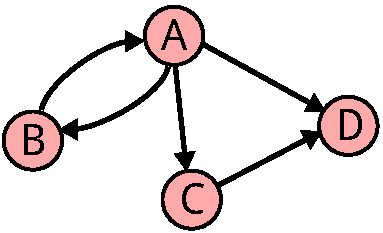
\includegraphics[width=4 cm]{asset/unweighted-directed.pdf}
  \end{figure}
\end{multicols} 
\end{center}
\end{frame}

\begin{frame}
\frametitle{Edge List (lanj.)}
\begin{itemize}
  \item Untuk graf berbobot, kita juga menyimpan bobot dari setiap \fedge.
\end{itemize}
\begin{center}
\begin{multicols}{2}
  $\begin{array}{l}
    <A, B, 3>, \\
    <A, C, 2>, \\
    <A, D, 5>, \\
    <B, A, 1>, \\
    <C, D, 8> 
  \end{array}$
  \break
  \begin{figure}
    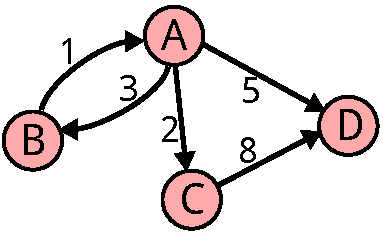
\includegraphics[width=4 cm]{asset/weighted-directed.pdf}
  \end{figure}
\end{multicols} 
\end{center}
\end{frame}

\begin{frame}
\frametitle{Implementasi Edge List}
\begin{itemize}
  \item Untuk implementasinya, kita membutuhkan struktur data sebuah \flist (atau \farray).
  \item Jelas bahwa memori yang dibutuhkan adalah $O(E)$, dengan $E$ adalah banyaknya \fedge pada keseluruhan graf.
  \newline
  \item Pada beberapa kasus, dilakukan pengurutan terhadap \fedgelist atau digunakan struktur data \foreignTerm{binary search tree}, yang memungkinkan implementasinya lebih efisien.
  Namun untuk saat ini kita tidak mempelajari hal tersebut.
\end{itemize}
\end{frame}

\begin{frame}
\frametitle{Analisis Edge List}
\begin{itemize}
  \item Kompleksitas menambah \fedge adalah $O(1)$.
  \item Bergantung dari implementasi, kompleksitas menghapus \fedge dan memeriksa keterhubungan sepasang \fnode bisa berupa $O(\log{E})$ sampai $O(E)$.
  \item Demikian juga untuk mendapatkan daftar tetangga dari \fnode, kompleksitasnya bisa berkisar antara $O(\log{E} + K)$ sampai $O(E)$, dengan $K$ adalah banyaknya tetangga dari \fnode tersebut.
\end{itemize}
\end{frame}

\begin{frame}
\frametitle{Keuntungan dan Kerugian Representasi Graf}
Untuk graf dengan $V$ \fnode dan $E$ \fedge: 
{\fontsize{9}{10}\selectfont\renewcommand{\arraystretch}{1.75}
\begin{center}
 \begin{tabular}{||r|c c c||} 
 \hline
 & \foreignTerm{Adj.Matrix} & \foreignTerm{Adj.List} & \foreignTerm{Edge List}\\
 \hline\hline
 Tambah \fedge & $O(1)$ & $O(1)$ & $O(1)$ \\ \hline
 Hapus \fedge & $O(1)$ & $O(K)$ & $O(E)$ \\ \hline
 Cek keterhubungan & $O(1)$ & $O(K)$ & $O(E)$ \\ \hline
 Daftar tetangga & $O(V)$ & $O(K)$ & $O(E)$ \\ \hline
 Kebutuhan memori & $O(V^2)$ & $O(E)$ & $O(E)$ \\ [0.5ex] 
 \hline
\end{tabular}
\end{center}
}
Dengan $K$ adalah banyaknya \fnode yang bertetangga dengan \fnode yang sedang kita periksa.
\end{frame}

\section{Penjelajahan Graf}
\frame{\sectionpage}

\begin{frame}
\frametitle{Penjelajahan Graf}
\begin{itemize}
  \item Representasi graf saja belum berguna karena belum dapat mencari informasi mengenai suatu graf
  \item \alert{Penjelajahan graf} merupakan penelusuran \fnode-\fnode pada suatu graf.
\end{itemize}
\end{frame}

\begin{frame}
\frametitle{Penjelajahan Graf (lanj.)}
\begin{itemize}
  \item Diberikan \fnode A dan \fnode B, apakah dari \fnode A kita dapat pergi ke \fnode B dengan \fedge yang ada?
  \item Permasalahan tersebut dapat diselesaikan menggunakan penjelajahan graf.
  \newline
  \item Terdapat 2 metode yang dapat digunakan, yaitu \newTerm{DFS} dan \newTerm{BFS}.
\end{itemize}
\end{frame}

\begin{frame}
\frametitle{DFS: Depth-First Search}
Penelusuran dilakukan terhadap \fnode yang lebih dalam terlebih dahulu (\foreignTerm{depth-first}). 

Sebagai contoh, misal terdapat graf berikut:

\begin{figure}
  \centering
  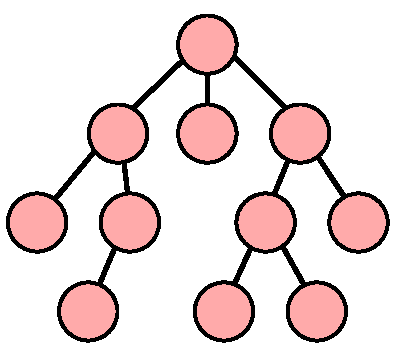
\includegraphics[width=4 cm]{asset/plain.pdf}
\end{figure}
\end{frame}

\begin{frame}
\frametitle{DFS: Depth-First Search (lanj.)}
Penelusuran secara DFS akan dilakukan dengan cara berikut:
\begin{figure}
  \centering
  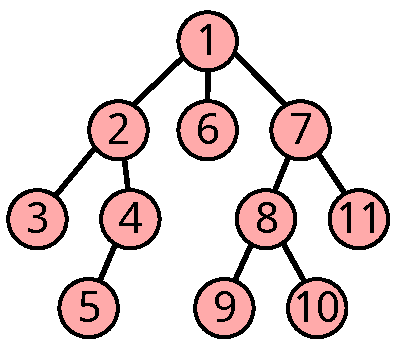
\includegraphics[width=4 cm]{asset/dfs.pdf}
\end{figure}
\begin{itemize}
  \item Angka pada \fnode menunjukkan urutan \fnode tersebut dikunjungi.
  \item \fNode 1 dikunjungi pertama, \fnode 2 dikunjungi kedua, dan seterusnya).
\end{itemize}
\end{frame}

\begin{frame}
\frametitle{Penelusuran DFS}
\begin{figure}
  \centering
  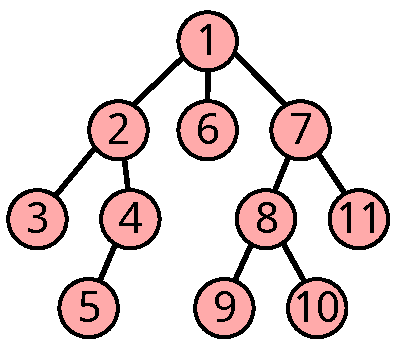
\includegraphics[width=4 cm]{asset/dfs.pdf}
\end{figure}
\begin{itemize}
  \item Dapat dilihat bahwa DFS mencoba menelusuri \fnode yang dalam terlebih dahulu.
  \item \fNode yang dekat dengan \fnode pertama (seperti \fnode 7 dan 8) akan dikunjungi setelah DFS selesai mengunjungi \fnode yang lebih dalam (seperti \fnode 3, 4, dan 5)
  \item Dalam pemrograman, DFS biasa dilakukan dengan rekursi atau struktur data \foreignTerm{stack}.
\end{itemize}
\end{frame}


\begin{frame}[fragile]
\frametitle{Implementasi DFS (Rekursif)}
Asumsikan:
\begin{itemize}
  \item Setiap \fnode dinomori dari 1 sampai $V$
  \item $adj(x)$ menyatakan himpunan tetangga dari \fnode $x$.
  \item $visited[x]$ bernilai $true$ hanya jika $x$ telah dikunjungi.
\end{itemize}
\begin{codebox}
  \Procname{$\proc{DFS}(curNode)$}
  \li \textbf{print} "mengunjungi $curNode$"
  \li  $visited[curNode] \gets true$
  \li \For \textbf{each} $adjNode \in adj(curNode)$ \Do
  \li   \If \textbf{not} $visited[adjNode]$ \Then
  \li     $\proc{DFS}(adjNode)$
        \End
      \End
\end{codebox}
\end{frame}

\begin{frame}[fragile]
\frametitle{Implementasi DFS (Stack)}
\begin{codebox}
  \Procname{$\proc{DFS}()$}
  \li \Comment Inisialisasi $stack$ sebagai stack kosong.
  \li $stack.push(initialNode)$
  \li $visited[initialNode] \gets true$
  \li \While \textbf{not} $stack.empty()$ \Do
  \li   $curNode \gets stack.top()$
  \li   $stack.pop()$
  \li   \textbf{print} "mengunjungi $curNode$"
  \li    $visited[adjNode] \gets true$
  \li   \For \textbf{each} $adjNode \in adj(curNode)$ \Do
  \li     \If \textbf{not} $visited[adjNode]$ \Then
  \li       $stack.push(adjNode)$
          \End
        \End
      \End
\end{codebox}
\end{frame}

\begin{frame}
\frametitle{BFS: Breadth-First Search}
Penelusuran \fnode pada graf dilakukan lapis demi lapis. 

Semakin dekat suatu \fnode dengan \fnode awal, \fnode tersebut akan dikunjungi terlebih dahulu. 

\begin{figure}
  \centering
  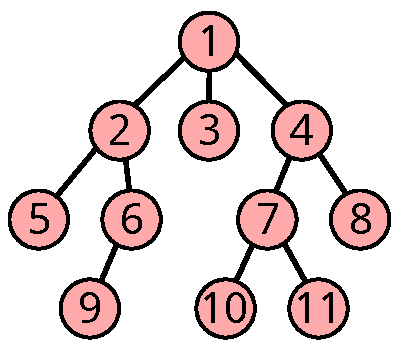
\includegraphics[width=4 cm]{asset/bfs.pdf}
\end{figure}
\end{frame}

\begin{frame}
\frametitle{Penelusuran BFS}
\begin{figure}
  \centering
  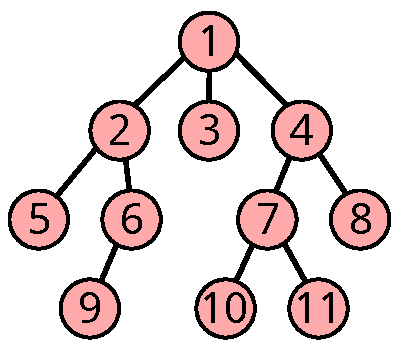
\includegraphics[width=4 cm]{asset/bfs.pdf}
\end{figure}
\begin{itemize}
  \item Angka pada gambar menunjukkan urutan \fnode tersebut dikunjungi.
  \item Dalam pemrograman, BFS biasa diimplementasikan dengan bantuan struktur data \foreignTerm{queue}.
\end{itemize}
\end{frame}

\begin{frame}[fragile]
\frametitle{Implementasi BFS}
\begin{codebox}
  \Procname{$\proc{BFS}()$}
  \li \Comment Inisialisasi $queue$ sebagai queue kosong.
  \li $queue.push(initialNode)$
  \li $visited[initialNode] \gets true$
  \li \While \textbf{not} $queue.empty()$ \Do
  \li   $curNode \gets queue.front()$
  \li   $queue.pop()$
  \li   \textbf{print} "mengunjungi $curNode$"
  \li   \For \textbf{each} $adjNode \in adj(curNode)$ \Do
  \li     \If \textbf{not} $visited[adjNode]$ \Then
  \li       $visited[adjNode] \gets true$
  \li       $queue.push(adjNode)$
          \End
        \End
      \End
\end{codebox}
\end{frame}

\begin{frame}
\frametitle{Analisis Kompleksitas}
\begin{itemize}
  \item Baik DFS maupun BFS sama-sama mengunjungi setiap \fnode tepat satu kali, dengan memanfaatkan seluruh \fedge.
  \item Kompleksitas dari kedua metode adalah:
  \begin{itemize}
    \item $O(V^2)$, jika digunakan \fadjacencymatrix.
    \item $O(V + E)$, jika digunakan \fadjacencylist.
    \newline
  \end{itemize}
  \item Penggunaan DFS atau BFS dapat disesuaikan dengan persoalan yang dihadapi.
\end{itemize}
\end{frame}

\begin{frame}
\frametitle{Contoh Permasalahan (lanj.)}
Pak Dengklek tinggal di kota A. Suatu hari, beliau ingin pergi ke kota B. Terdapat beberapa ruas jalan yang menghubungkan kota-kota dalam negara tempat beliau tinggal. Namun karena sudah tua, Pak Dengklek ingin melewati sesedikit mungkin ruas jalan untuk sampai ke kota B.
\newline\newline
Diberikan informasi mengenai struktur kota dan ruas jalan, tentukan berapa banyak ruas jalan yang perlu beliau lewati untuk pergi dari kota A ke kota B!
\end{frame}

\begin{frame}
\frametitle{Solusi}
\begin{itemize}
  \item Permasalahan ini dapat diselesaikan dengan BFS. 
  \item Karena sifat BFS yang menelusuri \fnode lapis demi lapis, maka dapat disimpulkan jika suatu \fnode dikunjungi, maka jarak yang ditempuh dari awal sampai \fnode tersebut pasti jarak terpendek.
  \item Hal ini selalu benar untuk segala graf tak berbobot, BFS selalu menemukan \foreignTerm{shortest path} dari suatu \fnode ke seluruh \fnode lainnya.
\end{itemize}
\end{frame}

\begin{frame}[fragile]
\frametitle{Implementasi Solusi}
\begin{codebox}
  \Procname{$\proc{shortestPath}(A, B)$}
  \li \Comment Inisialisasi $queue$ sebagai queue kosong.
  \li \Comment Inisialisasi array $visitTime$ dengan -1.
  \li $queue.push(A)$
  \li $visitTime[A] \gets 0$
  \li \While \textbf{not} $queue.empty()$ \Do
  \li   $curNode \gets queue.front()$
  \li   $queue.pop()$
  \li   \For \textbf{each} $adjNode \in adj(curNode)$ \Do
  \li     \Comment Jika $adjNode$ belum pernah dikunjungi...
  \li     \If $visitTime[adjNode] \isequal -1$ \Then
  \li       $visitTime[adjNode] \gets visitTime[curNode] + 1$
  \li       $queue.push(adjNode)$
          \End
        \End
      \End
  \li \Return $visitTime[B]$
\end{codebox}
\end{frame}

\section{Macam-Macam Graf}
\frame{\sectionpage}

\begin{frame}
\frametitle{Macam-Macam Graf}
\begin{itemize}
  \item Terdapat Graf yang memiliki suatu karakteristik khusus, sehingga penyelesaian masalah yang melibatkan graf ini dapat memanfaatkan karakter tersebut.
  \item Contoh macam-macam graf adalah \newTerm{tree}, \newTerm{directed acyclic graph}, dan \newTerm{bipartite graph}.
  \item Kali ini kita akan menyinggung \ftree dan \foreignTerm{directed acyclic graph}.
\end{itemize}
\end{frame}

\begin{frame}
\frametitle{Tree}
\begin{itemize}
  \item \fTree merupakan bentuk khusus dari graf.
  \item Seluruh \fnode pada \ftree terhubung (tidak ada \fnode yang tidak dapat dikunjungi dari \fnode lain) dan tidak terdapat \alert{cycle}.
  \item Banyaknya \fedge dalam sebuah \ftree pasti $V-1$, dengan $V$ adalah banyaknya \fnode.
\end{itemize}
\begin{center}
  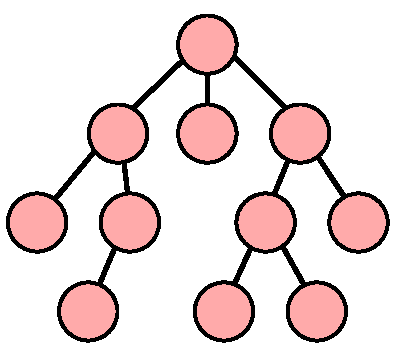
\includegraphics[width=3.5 cm]{asset/plain.pdf}
\end{center}
\end{frame}

\begin{frame}
\frametitle{Contoh Tree}
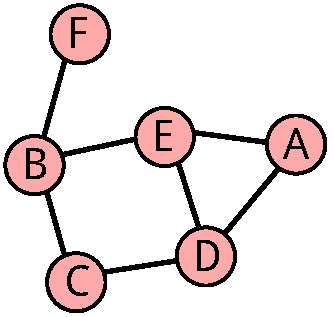
\includegraphics[width=3.5 cm]{asset/not-tree.pdf}
\hspace{\fill}
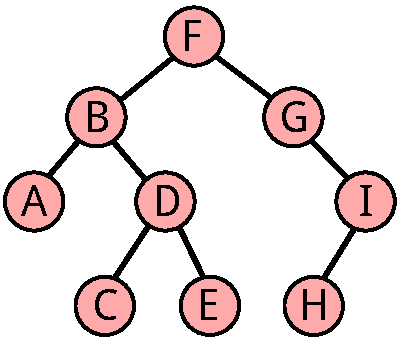
\includegraphics[width=4 cm]{asset/tree.pdf}
\newline\newline
Gambar kiri bukan \ftree karena memiliki \foreignTerm{cycle}, sedangkan gambar kanan merupakan \ftree. 
\end{frame}

\begin{frame}
\frametitle{Directed Acyclic Graph}
\begin{itemize}
  \item \foreignTerm{directed acyclic graph (DAG)} merupakan bentuk khusus dari \foreignTerm{directed} graf.
  \item DAG tidak memiliki \alert{cycle}.
  \item Berbeda dengan \ftree yang mana setiap \fnode harus dapat dikunjungi dari \fnode lainnya, sifat tersebut tidak berlaku pada DAG.
\end{itemize}
\begin{center}
  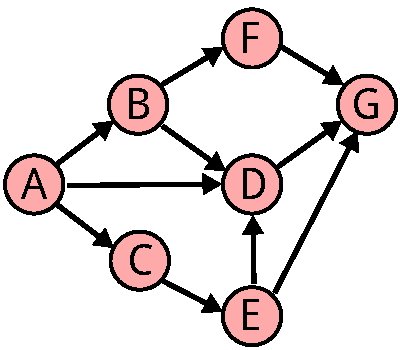
\includegraphics[width=4 cm]{asset/dag.pdf}
\end{center}
\end{frame}

\begin{frame}
\frametitle{Contoh Directed Acyclic Graph}
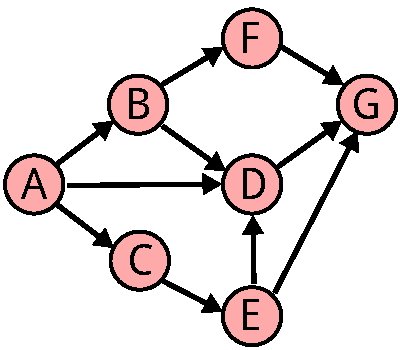
\includegraphics[width=4 cm]{asset/dag.pdf}
\hspace{\fill}
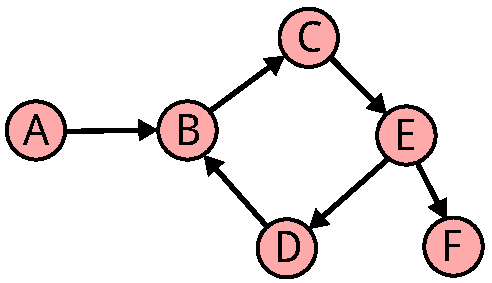
\includegraphics[width=5 cm]{asset/not-dag.pdf}
\newline\newline
Pada gambar di atas, gambar kiri merupakan DAG, sedangkan gambar kanan bukan DAG karena memiliki \foreignTerm{cycle}.
\end{frame}

\begin{frame}
\frametitle{Penutup}
\begin{itemize}
  \item Hampir setiap kompetisi pasti memiliki soal yang bertemakan graf.
  \item Mampu menguasai dasar penyelesaian masalah graf menjadi kemampuan penting dalam dunia kompetisi.
\end{itemize}
\end{frame}

\end{document}
